\chapter{自然语言处理}
\begin{introduction}
  \item Attention Mechanism
  \item Transformer
  \item BERT
  \item GPT
  \item Bi-Encoder
  \item Cross-Encoder
\end{introduction}

\section{注意力机制 (Attention Mechanism)}


\subsection{为什么要用多头注意力机制?}

通俗的解释是,Multi-head Attention会学习不同的 Q、K、V 子空间,因而能够将这种不同维度的信息综合起来,获得更好的performance。

\section{Transformer}

\begin{figure}[htbp]
  \centering
  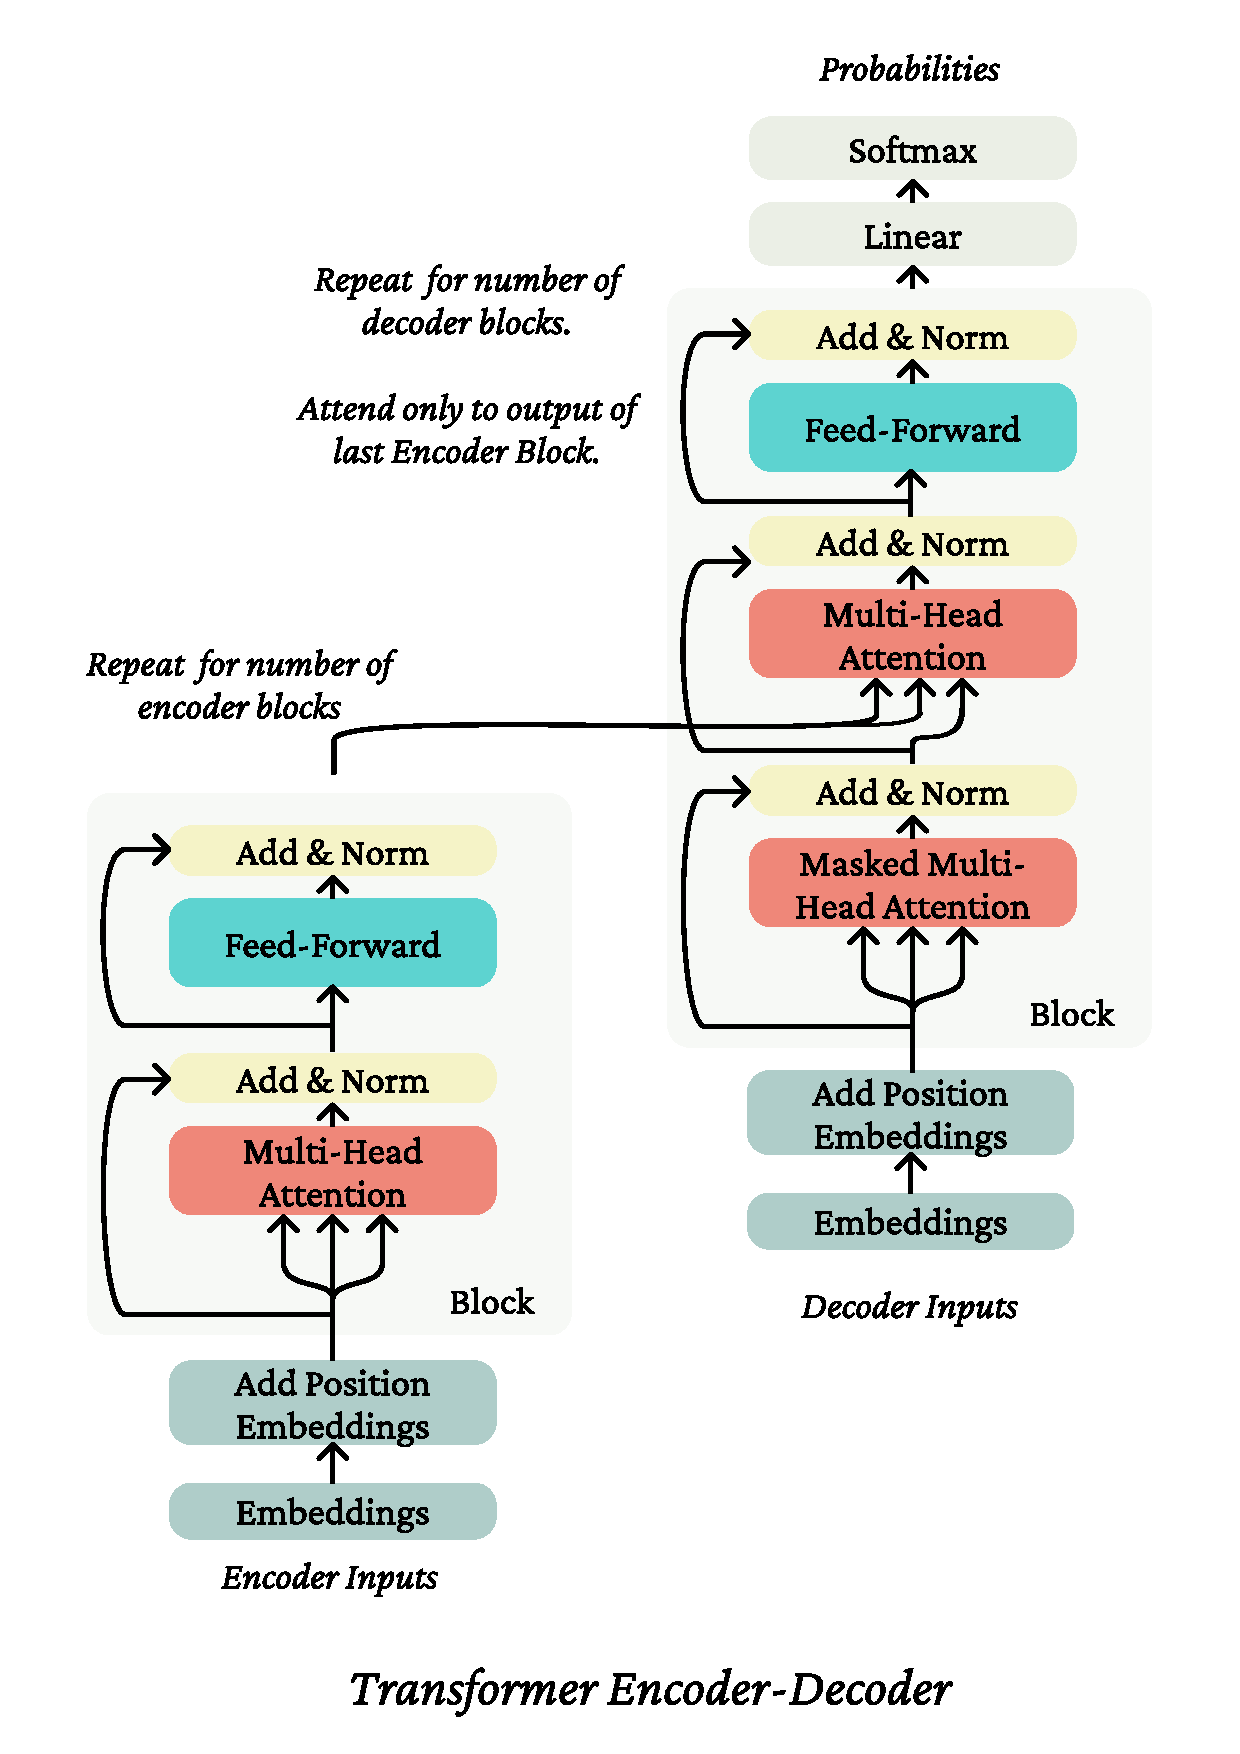
\includegraphics[width=0.6\textwidth]{transformer.pdf}
  \caption{Transformer架构 \label{fig:transformer}}
\end{figure}


\subsection{Batch Normalization 还是 Layer Normalization?}

\section{基于BERT的检索模型}

本章节将介绍两种业界常见的基于BERT的信息检索(Information Retrieval)模型:Bi-Encoder和Cross-Encoder。其中Bi-Encoder是双塔结构,主要用于信息的召回阶段;Cross-Encoder为单塔结构,主要用于召回后的精排或者粗排。

\subsection{Bi-Encoder}

\subsection{Cross-Encoder}
